\section{Durchführung}
\label{sec:Durchführung}
Im Versuch sollen der Ablenkungswinkel $\eta$ in Abhängigkeit von der Wellenlänge
des Lichts und der Innenwinkel $\phi$ einer Prismenecke gemessen werden. Es wird
die in Abbildung \ref{fig:geraet} dargestellte Messapparatur verwendet.

\begin{figure}[H]
  \centering
  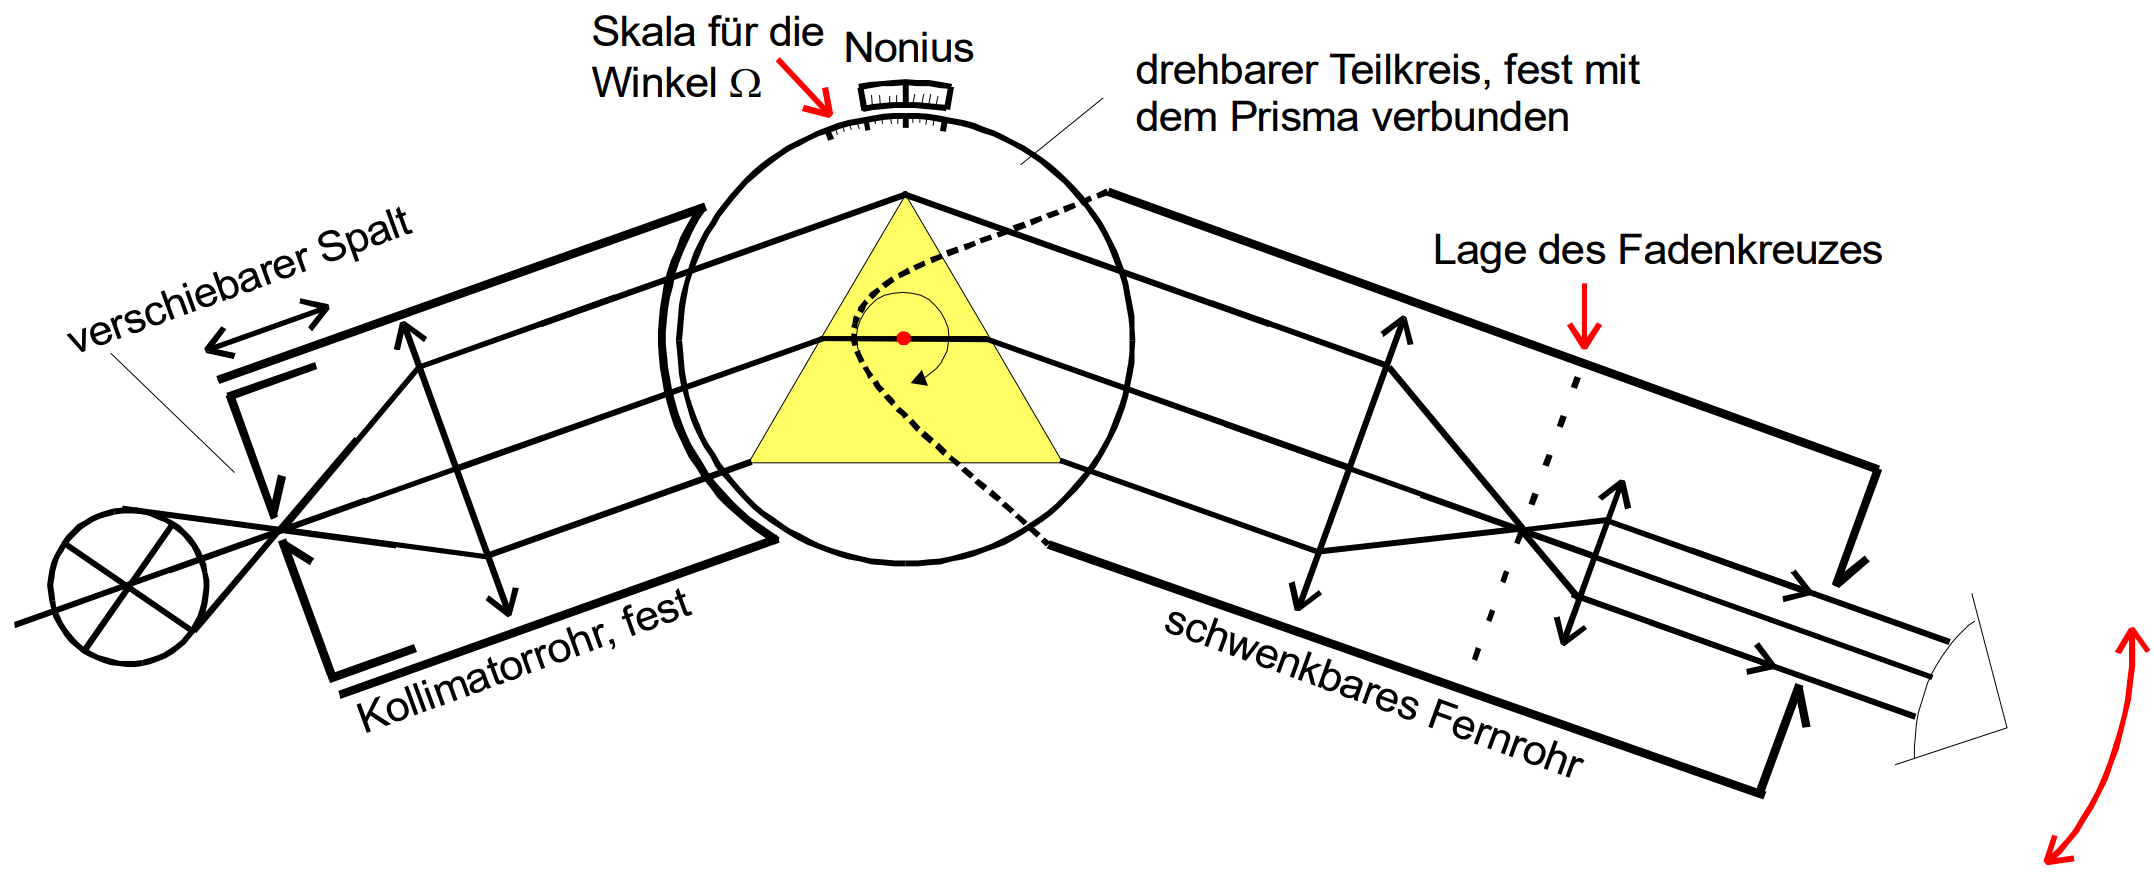
\includegraphics[height=5cm]{data/aufbau.png}
  \caption{Skizze der Messapparatur \cite{Versuchsanleitung}.}
  \label{fig:geraet}
\end{figure}

Aus einer Hg-Cd-Lampe fällt Licht auf einen Spalt, der in der Brennebene einer Linse
liegt, die den Strahl so fokussiert, dass ein paralleler Strahlengang auf das Primsa fällt.
Das Prisma besteht dabei aus Schwerflintglas 18. Nachdem das Licht im Prisma gebrochen oder vom
Prisma reflektiert wurde, kann es durch ein mit konstantem Abstand zum Prisma auf
einem Kreis bewegbaren Fernrohr mit dem Auge beobachtet werden. Die Schärfe des Bildes
kann am Fernrohr geregelt werden.

Für die Messung des Winkels $\eta$ wird für jede sichtbare Spektrallinie ein möglichst
paralleler Strahlengang im Prisma erzeugt, indem Prisma und Fernrohr so justiert werden,
dass das reflektierte Strahlenbündel genau mit der zu untersichenden Spektrallinie zusammenfällt.
Für jede Spektrallinie wird der Winkel notiert. Skizzen hierzu sind in den Abbildungen
\ref{fig:eta1} und \ref{fig:symmetrisch} zu sehen.

\begin{figure}[H]
  \centering
  \begin{subfigure}{0.48\textwidth}
    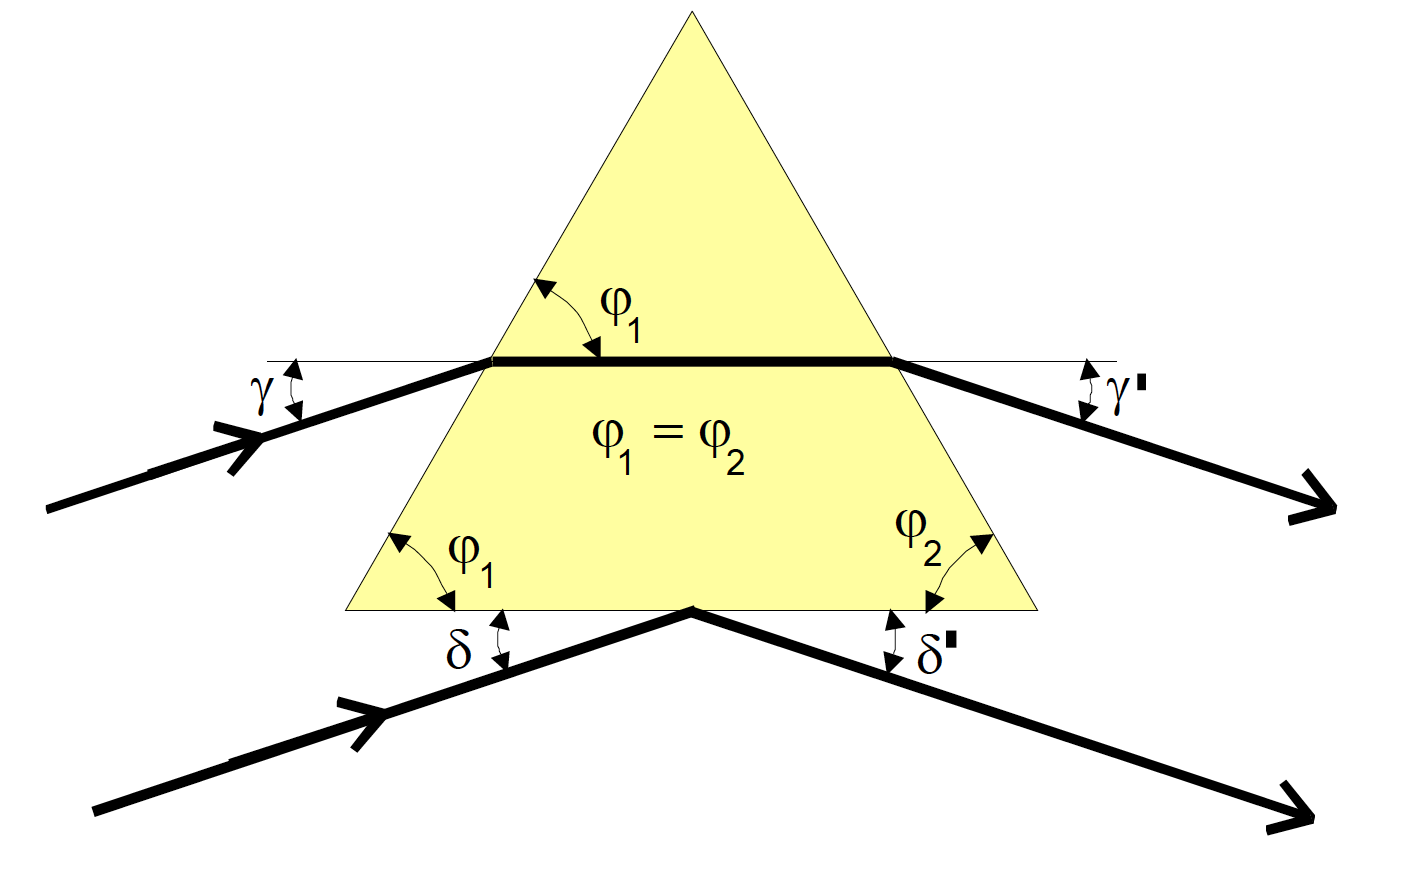
\includegraphics[height=5cm]{data/eta1.png}
    \caption{Skizze des gebrochenen und des reflektierten Strahls bei Symmetrischem
    Strahlenverlauf \cite{Versuchsanleitung}.}
    \label{fig:eta1}
  \end{subfigure}
  \begin{subfigure}{0.48\textwidth}
    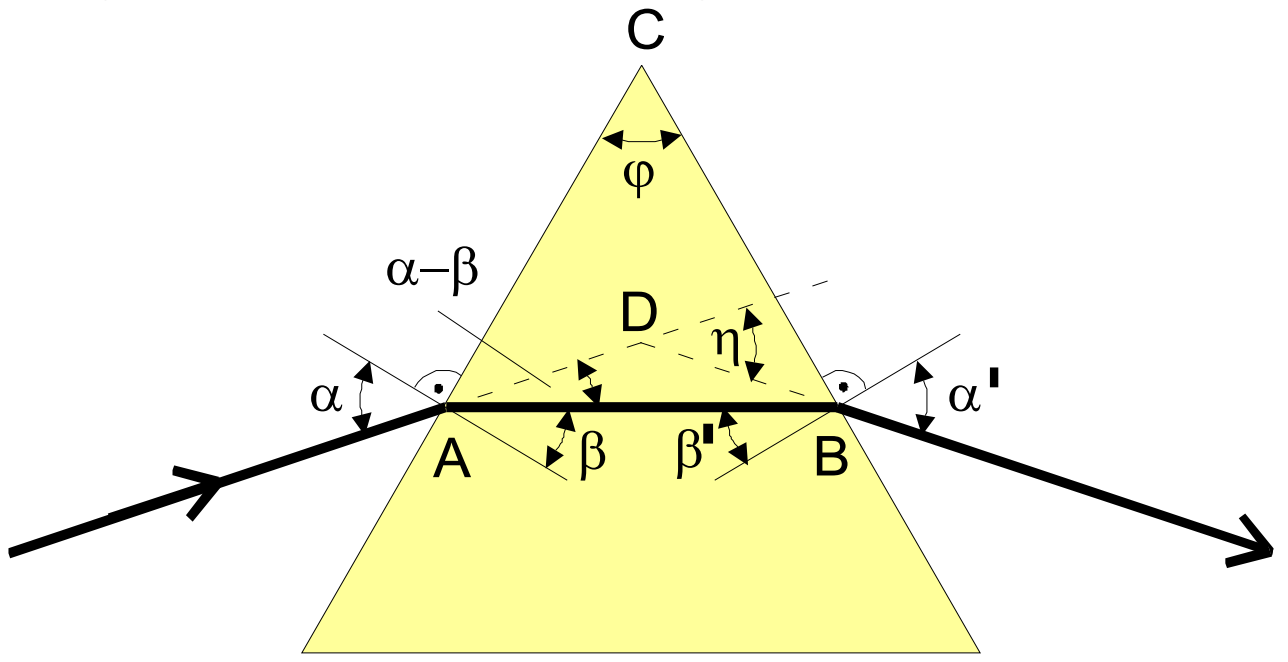
\includegraphics[height=5cm]{data/symmetrisch.png}
    \caption{Skizze des symmetrischen Strahlenverlaufs durch ein Prisma \cite{Versuchsanleitung}.}
    \label{fig:symmetrisch}
  \end{subfigure}
\end{figure}

Danach wird die gleiche Messung in Spiegelsymmetrischer Stellung des Prismas erneut
durchgeführt. Eine Skizze hierzu befindet sich in Abbildung \ref{fig:eta2}.
Aus den beiden bestimmten Winkeln kann schließlich der Winkel $\eta$ gemäß
\begin{equation}
  \eta=180°-(\Omega_{\symup{r}}-\Omega_{\symup{l}})
  \label{eqn:eta}
\end{equation}
berechnet werden.

\begin{figure}[H]
  \centering
  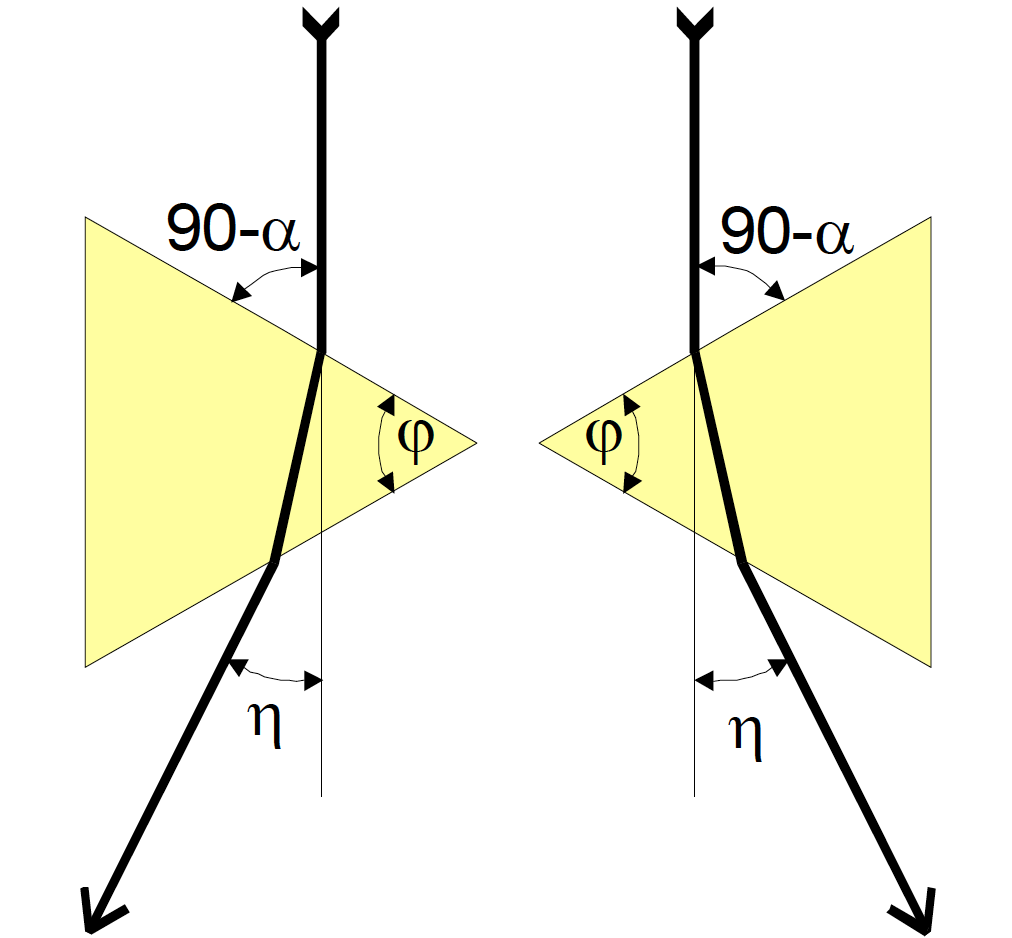
\includegraphics[height=5cm]{data/eta2.png}
  \caption{Skizze zur Bestimmung des Winkels $\eta$ aus zwei spiegelsymmetrischen Stellungen
  des Prismas \cite{Versuchsanleitung}.}
  \label{fig:eta2}
\end{figure}

Zur Bestimmung des Winkels $\phi$ einer Ecke des Prismas wird das Prisma mit dieser
Ecke in Richtung der Lampe positioniert und es wird auf beiden Seiten der Winkel gemessen,
unter dem Reflexion zu finden ist. Aus diesen beiden Winkeln kann der Winkel $\phi$
gemäß
\begin{equation}
  \phi=\frac{1}{2}(\phi_{\symup{r}}-\phi_{\symup{l}})
  \label{eqn:phi}
\end{equation}
berechnet werden. Eine Skizze hierzu befindet sich in Abbildung \ref{fig:phi}.
Die Messung wird für sieben leicht verschiedene Ausrichtungen des Prismas bestimmt.

\begin{figure}[H]
  \centering
  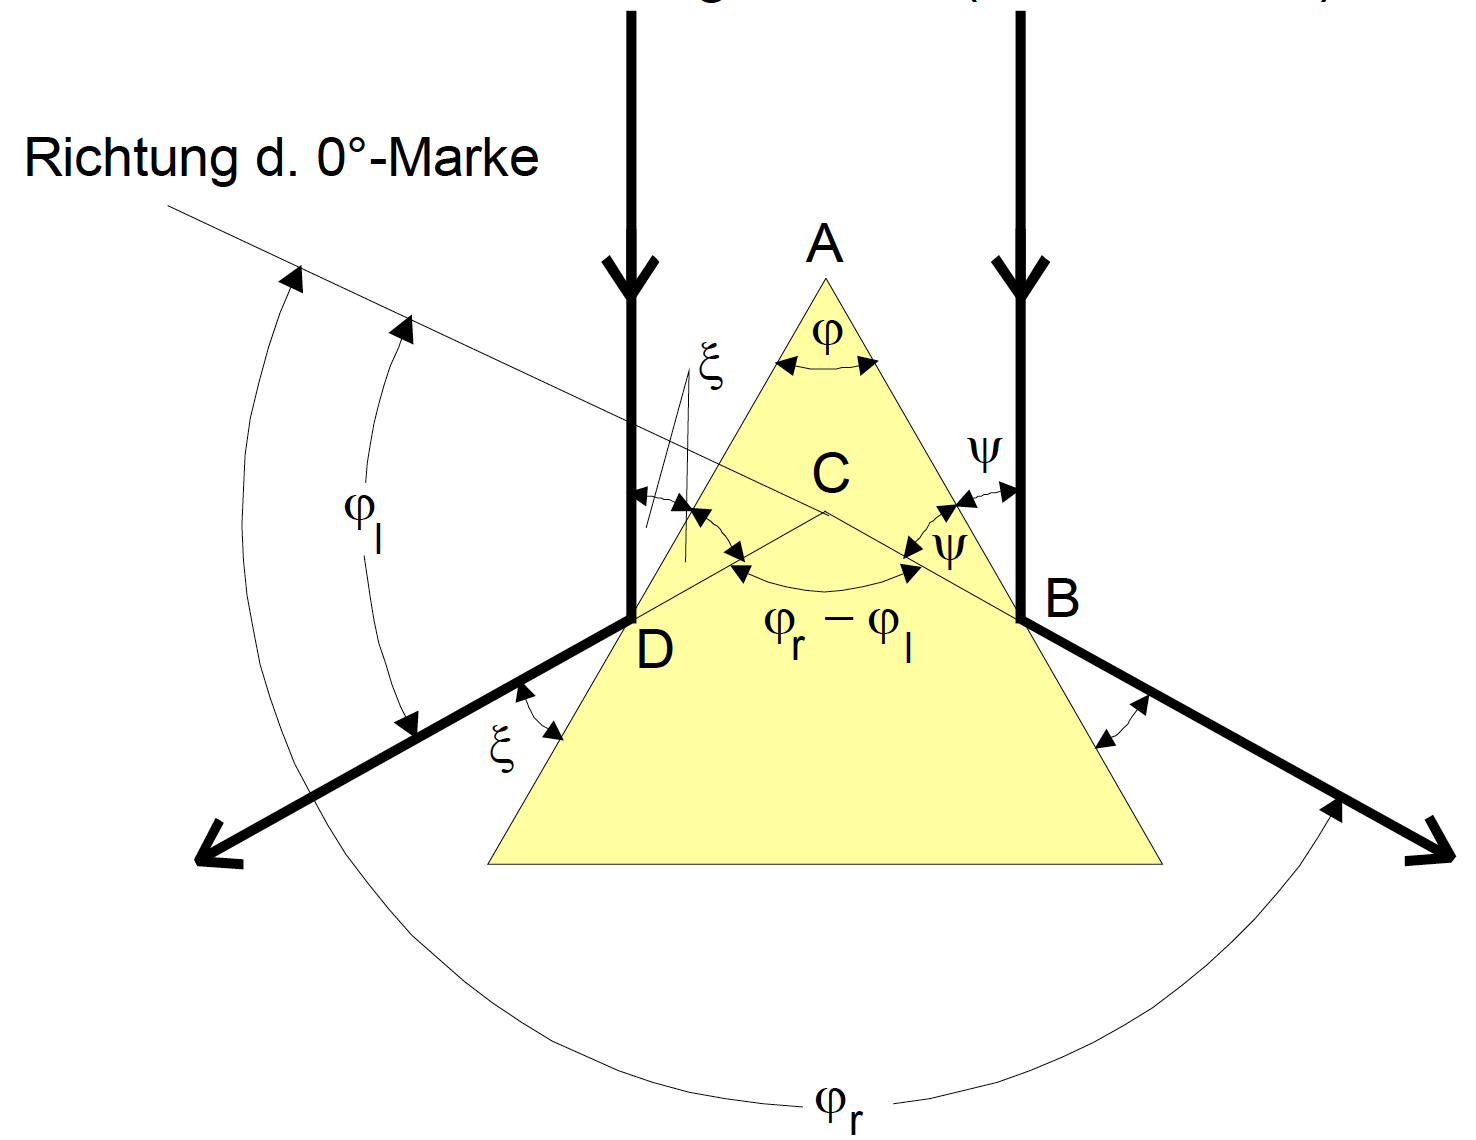
\includegraphics[height=5cm]{data/phi.png}
  \caption{Skizze zur Bestimmung des Winkels $\phi$ \cite{Versuchsanleitung}.}
  \label{fig:phi}
\end{figure}
